
%
% File: chap03.tex
% Author: Antigoni Kourou
% Description: The proposed approach
%
\let\textcircled=\pgftextcircled
\chapter{The proposed approach}
\label{chap:prop}

\initial{F}or transforming the text feedback into quantitative data, which will serve as input for analysis purposes, this paper proposes an approach as shown in Figure \ref{fig:pipe}. The pipeline consists of four main steps: \textit{pre-processing, feature identification, sentiment detection}  and \textit{data analysis}. Initially, the whole input of the pipeline is the huge corpus of text reviews stored in Neo4J database. This big amount of data is considered to be very noisy, therefore it will be cleaned up as be described in the following section. Features and sentiment are then identified in text based in sentence level. The output of these three stages consists of the quantitative sentiment scores for sentences of reviews and the features identified in them. This output will then be analyzed in the final stage, data analysis.  
%
%
%
\section{Pre-processing}
%
% ------------------------------------
The pipeline reads the text data from  Neo4J graph database, with the help of \textit{py2neo 2.0.8}\footnote{http://py2neo.org/2.0}, a toolkit for working with Neo4J from within Python applications, and it formulates the queries in Cypher \cite{panzarino2014learning}, the querying language for Neo4J graph database. In my work, the whole concept of the pipeline is developed in English, as the most used language in e-tourism websites and as the most popular language in the research field of opinion mining. The reviews in the corpus are read one by one and each of them is checked, rather it is written in the English language. For this purpose, the pipeline uses \textit{langdetect 1.0.1}\footnote{https://pypi.python.org/pypi/langdetect/1.0.1}, a language detection library ported from Google's language-detection. Thus, every time that the algorithm runs into a review not in English, it will ignore the review and continue to the next one. 
\begin{figure}[h!]
	\centering
	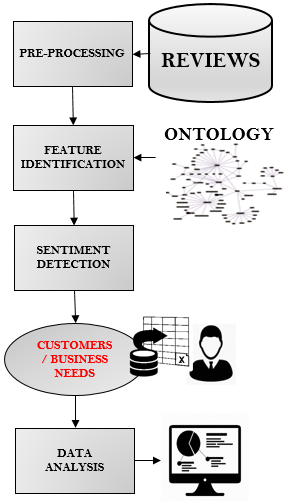
\includegraphics[height=0.5\textheight]{pipe}
	\caption{The proposed approach}
	\label{fig:pipe}
\end{figure} 
For each detected review in English, the algorithm will cut the text into sentences, using the NLTK Data package, which is based in English punctuation marks. The intention of this step is to detect the sentiment in sentence-level and to extract features within these sentences. From this action, results that a review has on average 5.1 sentences, where the maximum number of sentences per review found is 41 sentences. The total number of sentences in English, that form the dataset, is 302 081 sentences. For all of them, tokenization and lemmatization are performed to each sentence of the review. Tokenization is used for chopping the sentences into words, phrases, symbols and emoticons, each represented as a token. Lemmatization is the process of getting the root of the words, called lemmas, while ignoring its other forms as part of the speech. For tokenization the pipeline uses the \textit{TweetTokenizer}\footnote{http://www.nltk.org/api/nltk.tokenize.html} package, part of NLTK 3.0 Package and Twitter-aware designed, in order to be able to identify emoticons and adapt to new domains. On the other hand lemmatization is performed using \textit{WordNet 3.0}\footnote{https://wordnet.princeton.edu/}, a large lexical database for English terms and also part of NLTK 3.0 package. In WordNet nouns, verbs, adjectives and adverbs are grouped into sets of cognitive synonyms (synsets), each expressing a distinct concept \cite{miller1995wordnet}. The output of the pre-processing steps is a list of lemmas for each sentence, which will be used by the pipeline on its next stages.
%
\section{Feature identification}
As soon as each sentence in the corpus of reviews is represented as a list of lemmas, the ontology based approach is used to identify the accommodation features of each sentence.  The lists of related terms of the features is lemmatized in the same way as explained above, and the duplicates are removed. The lemmatization process aims to create a list of related lemmas for each feature in the ontology, which will then be used for feature identification in the sentences.
Thus, the feature identification step is a string match of the list of lemmas for every single sentence, with the list of related lemmas of every feature in the ontology. Considering that the ontology consists of many terms, this sample pipeline is trained to identify only six features that Airbnb asks the customers to manually rate as part of their feedback, namely \textit{accuracy, cleanliness, check-in, communication, location} and \textit{value}. 

When a word in the sentence is identified to be a feature, the algorithm jumps to the next word of the sentence. Within one sentence more than one feature can be identified, as well as features can be mentioned more than once. Therefore, for every possible feature match, a\textit{ match counter } variable, which keeps track of the features mentioned, is assigned to the sentence. Equation \ref{eq4} explains how the pipeline keeps track of the features mentioned per sentence. Here, the pipeline considers each sentence as independent and it ignores the logical connection between two sentences of the same review.
\begin{equation}
  Feature_i=\left\{
    \begin{array}{@{} l c @{}}
      k & \text{$feature$ mentioned k times} \\
      0 & \text{$feature$ not mentioned}
    \end{array}\right.
  \label{eq4}
\end{equation}


\section{Sentiment detection}
A very important part of the pipeline is the sentiment detection of sentences. The algorithm used for this purpose is VADER (Valence Aware Dictionary for Sentiment Reasoning) \footnote{https://pypi.python.org/pypi/vaderSentiment}, part of Python packages. VADER is a lexicon and rule-based sentiment analysis tool, that is specifically attuned to sentiments expressed in social media. For building the valence scores for sentiment intensity, VADER considers several well-known sources, such as ANEW, SentiWordNet 3.0 and SenticNet. These dictionaries include not only lexical features, but also grammatical and syntactical rules.
Therefore, VADER is able to deal with negation, capital letters, degree modifiers, emoticons, punctuation types, contrastive conjunctions (\textit{but, however}and slangs.  Based on the comparisons of 22 sentiment mining tools of the last decade, VADER is ranked as the best algorithm for comments and the second best for social networks \cite{ribeiro2015benchmark}. Some of its assigned scores are \textit{(good 0.7); (great 0.9434); (awesome	0.8306); (dirty -0.83066); (terrible -0.9434)} \footnote{The full lexicon can be found in: \textit{https:\/\/github.com\/cjhutto\/vaderSentiment\/tree\/master\/additional\_resources}}. In this paper, the pipeline uses VADER to return a sentiment score for every sentence of the review, which would afterwards serve as a discrete score for the identified features in that sentence. So, the algorithm returns a discrete score of sentiment per sentence, which we have to distribute to the features mentioned in it. Considering that in one sentence, more than 1 feature can be identified or the same feature can be identified more than once as mentioned above, a probabilistic model is developed. When calculating the sentiment we have four granularity levels to deal with: feature, sentence, review and listing. Starting from the top level, we have 2 356 listings, \textit{L = \{ L\textsubscript{0}, L\textsubscript{1},  L\textsubscript{2} ... L\textsubscript{2355} \}}. Each listing in this corpus can be represented by the ID of the listing in the database \textit{listing\_id}. Every listing from this set has a number of reviews, which varies from one listing to the other and is identified from ID of the review \textit{R\textsubscript{listing} = \{ R\textsubscript{0}, R\textsubscript{1},  R\textsubscript{2} ... R\textsubscript{r} \}}. For a single review of a certain listing would be \textit{R\textsubscript{listing, review}}. This review is composed by a number of sentences \textit{S\textsubscript{listing, review} = \{S\textsubscript{0}, S\textsubscript{1}, S\textsubscript{2} ... S\textsubscript{s}\}}. 
In each of these sentences, the pipeline is trained to identify six accommodation features \textit{F = \{accuracy, check-in, cleanliness, communication, location, value\}}, as explained in the previous section. When the sentiment of a sentence is detected, it does not particularly refer to a certain feature. Therefore, based on the sentiment of the sentence where the feature is mentioned, we have to calculate the feature's sentiment.
<<<<<<< HEAD
\ref{eq3.2} shows that the sentiment score (SS) of a feature in sentence level depends on the SS of the sentence itself and the feature weights, which is the number of times the feature is mentioned in this sentence compared to the total number of features mentioned in it.
=======
Equation \ref{eq3.2} shows that the sentiment score (SS) of a feature in sentence level depends on the SS of the sentence itself, the number of times a feature is mentioned in this sentence and the total number of features mentioned in it.
>>>>>>> ff3c390380db8e5c1529427a5b56e71f97095fa2
%
% ----------------FORMULA--------------------
%
\begin{equation}
SS_{(sentence,feature)} = \frac{k}{n} * SS_{sentence}
\label{eq3.2}
\end{equation}
where \textit{k} is the number of times the feature is mentioned in the sentence and \textit{n} the total number of features mentioned in this sentence. Afterwards, the SS for a feature of a review would be the average SS for that feature of all the sentences of that review. Similarly, the SS for a feature of a listing is the average SS for that feature of the reviews of that listing.
The calculation of sentiment scores of the features in sentence level is done as part of the sentiment detection phase of the pipeline and it is repeated for every single sentence. For clarifying its use, let us take an example. Considering the reviews of a random listing, i.e. 24328,  \textit{R\textsubscript{24328, 10146}} would represent the review:
\begin{quote}
\textit{We had a great stay at Joe's. The handy guide to the house and neighborhood was much appreciated, as were Joe's clear instructions for checking in while he was away. The house was comfortable and eclectic, full of personal character.}
\end{quote}
Now, let's focus on the second sentence of this review. In this sentence, can be identified three features \textit{check-in, communication,} and \textit{location} each once, thus for each of them \textit{k} would be 1 and \textit{n} would be 3. Figure \ref{fig:sent} shows the results of the pipeline for this case. Then based on this output the sentiment of features in review and listing level is calculated in a later phase, as part of data analysis.
\begin{figure}[h!]
	\centering
	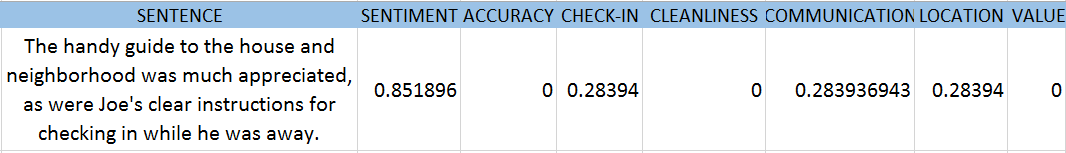
\includegraphics[height=0.1\textheight]{example_pip}
	\caption{Example of the probabilistic sentiment results}
	\label{fig:sent}
\end{figure}
%
\section{Data analysis}
% 
% will explain the analysis process using Pandas for different cases! 
%
The last step of the pipeline and the most interesting one for service providers and businesses is data analysis. Up to here, we saw the pipeline processing all the text data step by step and transform them into meaningful sentiment scores, for each sentence and each accommodation feature of the reviews. The output of these phases is a Comma Separated Vector (.csv) file, consisting of all listings, all listings' reviews, its respective sentences and the sentiment for the identified features on these sentences. This scores are analyzed with Pandas\footnote{http://pandas.pydata.org/}, an open source library providing high-performance, easy-to-use data structures and data analysis tools for Python. The workspace  of analysis and visualization of results is Jupyter Notebook, a web application, that allows users to create and share documents that contain  interactive code, equations, visualizations and explanatory text. For transforming the sentiment scores of reviews and listings into star ratings, the following coding scheme is used:

\tiny
\begin{lstlisting}[language=python]
	if (Sentiment < -0.75):	stars = 1
  			elif (-0.75 <= Sentiment < -0.5): stars = 1.5
    			elif (-0.5 <= Sentiment < -0.25): stars = 2
    				elif (-0.25 <= Sentiment < 0.0): stars = 2.5
            				elif (Sentiment==0.0): stars = 3
    		elif (0.0 < Sentiment < 0.25): stars = 3.5
    			elif (0.25 <= Sentiment < 0.5): stars = 4
    				elif (0.5 <= Sentiment < 0.75): stars = 4.5
    					elif (0.75 <= Sentiment): stars = 5
\end{lstlisting}
\normalsize
The rating 3 is assigned only is cases when no sentiment is detected in the sentence, otherwise we intend to cluster them as positive or negative, rather than neutral. The data  analysis in this step includes calculation and visualization of sentiment scores per reviews and listings, frequency of features mentioned in reviews, ranking of listings based on overall sentiment or based on sentiment of one or more specific features, cancellation rates of listings, computation and comparisons of sentiment scores from the pipeline with the ratings of Airbnb and so further. Naturally, the analysis can be extended and customized to match the specific interest of the service providers or the customers. The main results of this analysis will be explored in the section of Results, followed by the implementation of pipeline, according to its usefulness for service providers and customers respectively. 